\documentclass[14pt]{beamer}

\usetheme{Madrid}

% Add frame numbers
\setbeamertemplate{page number in head/foot}[framenumber]

\usepackage{amsmath, amssymb}
\usepackage{tikz}
\usepackage{bm}
\usepackage{outlines}   % For multilevel lists using the outline environment
\usepackage{natbib}
\usepackage{subcaption}
\usepackage{comment}    % for \begin{comment} ... \end{comment}

\renewcommand*{\bibfont}{\scriptsize}

\newcommand{\CMA}{Causal Mediation Analysis}

\newcommand{\bE}{\mathbb{E}}
\newcommand{\bF}{\mathbb{F}}
\newcommand{\bG}{\mathbb{G}}
\newcommand{\bV}{\mathbb{V}}
\newcommand{\I}{\mathcal{I}}

\newcommand{\ess}{ESS_*}
\newcommand{\esst}{ESS_2}
\newcommand{\esso}{ESS_1}
\newcommand{\essi}{ESS_\infty}
\newcommand{\essp}{ESS_P}


\newcommand{\eh}{\hat{\bE}}
\newcommand{\et}{\tilde{\bE}}


\title[]{Adaptive Importance Sampling}
\author{William Ruth}
\institute[]{Mount Royal University}
\date{\vspace{-3cm}}
% \titlegraphic{
\includegraphics[width=2cm]{Logos/CANSSI_Logo.png} \hspace{2cm} 
\includegraphics[width=4cm]{Logos/Logo_UdeM-CMJN.jpg}}


\begin{document}

\begin{frame}
    \titlepage
\end{frame}


\begin{frame}{Outline}
    \begin{outline}
        \1 Importance sampling \newline
        \1 Measuring performance
            \2 Effective sample size \newline
        \1 Improving performance
            \2 Stochastic approximation

    \end{outline}
\end{frame}


\begin{frame}{Importance Sampling}
    \begin{outline}
        \1 Need to compute an expected value
            \2 $\bE_F \varphi(X) =: \mathcal{I}$
        \1 Can't do the sum/integral \newline

        \1 Monte Carlo approximation
            \2 Simulating from $F$ might be hard
    \end{outline}
    \begin{equation*}
    \end{equation*}
\end{frame}

\begin{frame}{Importance Sampling}
    \begin{outline}
        \1 Introduce ``proposal distribution'', $G$:
    \end{outline}
    \begin{align*}
        \bE_F \varphi(X) &=  \bE_G \left[ \varphi(X) \cdot \frac{f(X)}{g(X)} \right] \\
        &=  \bE_G \left[ \varphi(X) \cdot w(X) \right]
    \end{align*}
    \begin{outline}
        \1 $G$ can be nearly anything*
            \2 *Some choices will be better than others
    \end{outline}
\end{frame}

\begin{frame}
    \frametitle{Importance Sampling}
    Option 1 (``Ideal'' Monte Carlo):
    \begin{outline}
        \1 Generate $X_1,\ldots, X_N \overset{iid}{\sim} \bF$
        \1 Estimate $\I$ with $\tilde{E} := \frac{1}{N} \sum \varphi (X_i)$
            \2 We often can't actually do this \newline
    \end{outline}
    Option 2 (Importance Sampling): 
    \begin{outline}
        \1 Generate $X_1, \ldots, X_N \overset{iid}{\sim} \bG$
        \1 Estimate $\I$ with $\hat{E} := \frac{1}{N} \sum w(X_i) \varphi (X_i)$
    \end{outline}
\end{frame}



\begin{frame}{Example: Standard Normal}
    \begin{outline}
        \1 $f$ standard normal 
        \1 $\varphi(X) = X^2$ \newline

        \1 Try some proposals:
            \2 $G_1 \sim N(0, 2^2)$
            \2 $G_2 \sim N(0, 0.5^2)$ \newline
        \1 Use $M=1000$ samples from proposal
            \2 $\hat{\bE}_1 = 0.99$, $\hat{\text{SD}} = 1.97$
            \2 $\hat{\bE}_2 = 1.10$, $\hat{\text{SD}} = 2.32$
    \end{outline}    
\end{frame}

\begin{frame}{Example: Standard Normal}
    \centering
    
\includegraphics[height=0.9\textheight, width=0.9\textwidth, keepaspectratio]{Figures/Wt Hist.pdf}
\end{frame}

\begin{frame}{Importance Sampling}
    \begin{outline}
        \1 Nothing obviously wrong with the $G_1$ weights
        \1 $G_2$ weights dominated by one large value \newline

        \1 We can make this difference precise
    \end{outline}
\end{frame}


\begin{frame}
    \frametitle{Effective Sample Size}
    \begin{outline}
        \1 Effective sample size measures the sample efficiency of importance sampling relative to ``ideal'' Monte Carlo
    \end{outline}
    \begin{gather*}
        \ess := N \cdot \frac{\bV \tilde{E}}{\bV \hat{E}}
    \end{gather*}
\end{frame}

{
\setbeamertemplate{itemize subitem}{\(\rightarrow\)}

\begin{frame}
    \frametitle{Effective Sample Size}
    \begin{outline}
        \1 If we choose a bad proposal, $\bV \hat{E}$ will be large
            \2 $\ess$ will be small \newline
        
        \1 If we choose a good proposal, $\ess \approx N$ \newline

        \1 It's possible to choose $\bG$ such that $\bV \hat{E} < \bV \tilde{E}$
            \2 $\ess > N$
            \2 This is why importance sampling is called a variance reduction technique
    \end{outline}
\end{frame}
}

\begin{frame}
    \frametitle{Effective Sample Size}

    \begin{outline}
        \1 Problem: If we can't even evaluate $\eh$, we probably can't get $\bV \eh$ \newline

        \1 We need ways to estimate $\ess$
    \end{outline}

\end{frame}



\begin{frame}
    \frametitle{Effective Sample Size}

    \begin{outline}
        \1 The most popular estimator for $\ess$ is
    \end{outline}
    \begin{gather*}
        \esst := \frac{[\sum w(X_i)]^2}{\sum w(X_i)^2}
    \end{gather*}
    \begin{outline}
        \1 This can be derived directly from $\ess$ with $\varphi(X) = X$ and some very strong simplifying assumptions
    \end{outline}
\end{frame}

\begin{frame}
    \frametitle{Effective Sample Size}

    \begin{outline}
        \1 This doesn't really look like it has anything to do with sample sizes, however:
        \2 If all weights are equal, $\esst = N$
        \2 If there are $k$ non-zero weights that are all equal, $\esst = k$ \newline

        \1 Problem: $\esst$ doesn't depend on $\varphi$
            \2 This is actually true for most ESS formulas
    \end{outline}
\end{frame}

\begin{frame}
    \frametitle{Aside: Self Normlization}

    \begin{outline}
        \1 Sometimes, we only know the target density up to a proportionality constant
            \2 E.g. Simulating from posterior distributions \newline

        \1 Use this one simple trick:
        \1 Divide each weight by the sum of the weights
            \2 Each weight is now in $(0,1)$, and they sum to 1
            \2 Unknown proportionality constant cancels \newline
        
        \1 Self-normalized importance sampling
    \end{outline}
\end{frame}

\begin{frame}
    \frametitle{Aside: Self Normlization}

    \begin{outline}
        \1 Write $\bar{w}_i$ for the $i$th normalized weight
            \2 Many ESS formulas assume that weights have been normalized \newline
        
        \1 Normalizing often simplifies formulas
        \1 E.g. $\esst = (\sum \bar{w}_i^2)^{-1}$

    \end{outline}
\end{frame}

\begin{frame}
    \frametitle{Aside: Self Normlization}

    \begin{outline}
        \1 Unfortunately, normalizing also makes $\eh$ biased
            \2 Still consistent for $\I$ \newline
        
        \1 For the rest of today, we will work with normalized weights
    \end{outline}
\end{frame}


\begin{frame}
    \frametitle{Effective Sample Size}

    \begin{outline}
        \1 I said earlier that $\esst$ is based on strong assumptions about the weights
        \1 Another way to motivate $\esst$ is based on the discrete uniform distribution \newline
        
        \1 Best case for IS is when all weights are equal
            \2 I.e. Weights $\sim$ discrete uniform
        \1 The farther we are from this ideal, the worse our ESS should be
        \1 Different distances give us different ESS
    \end{outline}
    

\end{frame}


\begin{frame}
    \frametitle{Effective Sample Size}

    \begin{outline}
        \1 $\esst$ comes from the $\mathcal{L}^2$ distance \newline
        
        \1 $\mathcal{L}^\infty$ gives us something quite different:        
    \end{outline}
    \begin{gather*}
        \essi := \frac{1}{\max \bar{w}_i}
    \end{gather*}
    

\end{frame}


\begin{frame}
    \frametitle{Effective Sample Size}

    \begin{outline}
        \1 We could also use $\mathcal{L}^1$   
    \begin{gather*}
        \esso := -N \sum \bar{w}_i \cdot I(\bar{w}_i > 1/N) + N^+ + N,
    \end{gather*}
        where $N^+$ is the number of weights larger than $1/N$ \newline

        \1 One last version of ESS, based on entropy instead of distances:
        \begin{gather*}
            \essp := \exp \left[ - \sum \bar{w}_i \log \bar{w}_i \right]
        \end{gather*}
        (Called perplexity)

    \end{outline}
    

\end{frame}

\begin{frame}
    \frametitle{Effective Sample Size}

    \begin{outline}
        \1 All these formulas look quite different \newline

        \1 However, all satisfy the properties from earlier:
            \2 If all weights are equal, $\text{ESS}=N$
            \2 If there's $k$ equal non-zero weights, $\text{ESS}=k$ \newline

    \end{outline}
    

\end{frame}

\begin{frame}
    \frametitle{Effective Sample Size}

    \begin{outline}
        \1 Which ESS should we use? \newline
        \1 Some comparisons in the literature: 

            \2 \citet{Mar16} found that $\esst$ and $\essi$ tend to bracket $\ess$ in a small simulation study
            \2 \citet{Mar25} found that it may be better to use $\mathcal{L}^p$-based ESS with $p$ as high as 8, depending on the scenario; also from small simulation studies
    \end{outline}
\end{frame}

\begin{frame}
    \frametitle{Adaptive Importance Sampling}

    \begin{outline}
        \1 Instead of using ESS to measure the performance of a single proposal, use it to find a good proposal \newline

        \1 Adaptive importance sampling involves finding an optimal proposal for a given problem
            \2 Different ESS formulas give us different measures of optimality
        \1 Perform optimization using stochastic approximation
    \end{outline}
\end{frame}


{

\setbeamertemplate{itemize subitem}{\(\rightarrow\)}


\begin{frame}
    \frametitle{Aside: Stochastic Approximation}

    \begin{outline}
        \1 Stochastic approximation was proposed by \citeauthor{Rob51} in 1951 for finding roots of functions with noise \newline

        \1 The next year, \citeauthor{Kie52} pointed out that this could find roots of gradients
            \2 Optimization of functions with noise
    \end{outline}
\end{frame}


\begin{frame}
    \frametitle{Aside: Stochastic Approximation}

    \begin{outline}
        \1 A root of $f(x)$ is a fixed point of $x + f(x)$
            \2 Use fixed point iteration for root finding
        \begin{gather*}
            x_{n+1} = x_n + f(x_n)
        \end{gather*}
        \1 \citeauthor{Rob51} showed that this recursion still works when you replace $f(x_n)$ with $\hat{f} (x_n) = f(x_n) + \varepsilon$
        \1 Also need a dynamic step size
    \end{outline}
 
\end{frame}


}


\begin{frame}
    \frametitle{Aside: Stochastic Approximation}
    \begin{outline}
        \1 The main reason we're interested in this method is to take $f$ as a gradient
            \2 Now, we're doing optimization \newline
        
        \1 Many functions of interest don't have analytical gradients
        \1 \citet{Kie52} suggested using a finite difference approximation
    \end{outline}
\end{frame}


\begin{frame}
    \frametitle{Aside: Stochastic Approximation}
    \begin{outline}
        \1 Fixed-point iteration for root finding
    \end{outline}
    \begin{gather*}
            x_{n+1} = x_n + f(x_n)
    \end{gather*}
\end{frame}



\begin{frame}
    \frametitle{Aside: Stochastic Approximation}
    \begin{outline}
        \1 \citet{Rob51}
    \end{outline}
    \begin{gather*}
            x_{n+1} = x_n + a_n \hat{f}(x_n)
    \end{gather*}
\end{frame}


\begin{frame}
    \frametitle{Aside: Stochastic Approximation}
    \begin{outline}
        \1 \citet{Rob51} for optimization
    \end{outline}
    \begin{gather*}
            x_{n+1} = x_n + a_n \widehat{\nabla f}(x_n)
    \end{gather*}
\end{frame}

\begin{frame}
    \frametitle{Aside: Stochastic Approximation}
\begin{outline}
        \1 \citet{Kie52}
    \end{outline}
    \begin{gather*}
            x_{n+1} = x_n + a_n \left[ \frac{\hat{f}(x_n + c_n) - \hat{f}(x_n - c_n)}{2c_n} \right]
    \end{gather*}
\end{frame}


\begin{frame}
    \frametitle{Aside: Stochastic Approximation}
    \begin{outline}
        \1 Disclaimer: The theory and practice of stochastic approximation has developed since the 50s \newline

        \1 E.g. Stochastic gradient descent, Polyak-Ruppert averaging, projection
    \end{outline}
\end{frame}


\begin{frame}
    \frametitle{Adaptive Importance Sampling}

    \begin{outline}
        \1 Let's combine the idea of effective sample size with stochastic approximation \newline
    \end{outline}
      \setbeamertemplate{enumerate items}[default]

    \begin{enumerate}
        \item Choose an ESS measure and a parametric family of proposals
        \item Use stochastic approximation to maximize the chosen ESS
        \item Profit
    \end{enumerate}
\end{frame}


\begin{frame}{Example: Normal Scale Family}
    \begin{outline}
        \1 Let's revisit the simple example from earlier
        \1 $f$ standard normal \newline

        \1 Proposal family: $\{ N(0, \sigma^2) \}$
    \end{outline}    
\end{frame}

\begin{frame}{Example: Normal Scale Family}
    \begin{outline}
        \1 Rather than choosing one ESS, I want to compare them \newline

        \1 Use stochastic approximation to optimize over $\sigma > 0$.
    \end{outline}    
\end{frame}


\begin{frame}{Example: Normal Scale Family}
    \begin{outline}
        \1 Rather than choosing one ESS, I want to compare them \newline

        \1 Use stochastic approximation to optimize over $\sigma > 0$.
    \end{outline}    
\end{frame}

\begin{frame}{Example: Normal Scale Family}
    \centering
    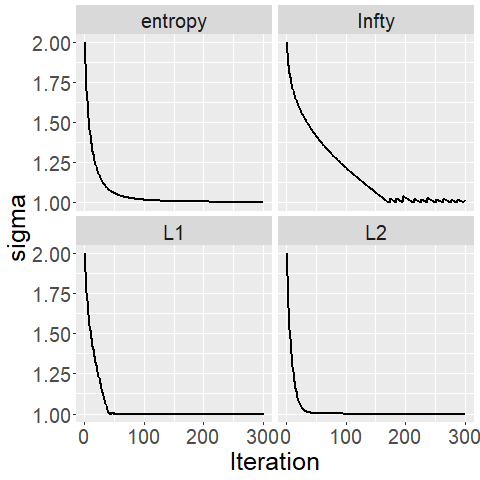
\includegraphics[height=0.8\textheight, width=0.9\textwidth, keepaspectratio]{Figures/New/Normal SA.png}
\end{frame}

\begin{frame}{Example: T Degrees of Freedom}
    \begin{outline}
        \1 Next, let's do something a little more interesting
        \1 $f$ standard normal \newline

        \1 Proposal family: $\{ T_n: n>0 \}$
    \end{outline}  
\end{frame}

\begin{frame}{Example: T Degrees of Freedom}
    \centering
    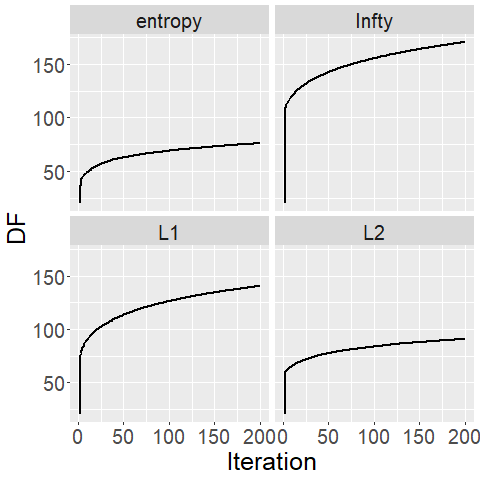
\includegraphics[height=0.8\textheight, width=0.9\textwidth, keepaspectratio]{Figures/New/T SA.png}
\end{frame}


\begin{comment}

% \begin{frame}{Example: Mystery Target}
%     \centering
%     
\includegraphics[height=0.7\textheight, width=0.9\textwidth, keepaspectratio]{Figures/Wt Hist.pdf} \newline
%     \begin{outline}
%         $ESS_1 \approx 662$ \hspace{2.5cm} $ESS_2 \approx 54$
%     \end{outline}
% \end{frame}

\begin{frame}{Importance Sampling}
    \begin{outline}
        \1 Problem: Low ESS $\rightarrow$ hard to estimate means \newline
        \1 But ESS is based on means
            \2 \citep{Cha18}
    \end{outline}
\end{frame}

% \begin{frame}{Importance Sampling}
%     \begin{outline}
%         \1 Consider $\varphi(X) = X$
%             \2 I.e. $\bE_F \varphi(X) = \bE_F(X)$ \newline
%         \1 $\hat{\bE} = \sum_i \frac{X_i w(X_i)}{M}$, $X_i \overset{\mathrm{iid}}{\sim} G$ \newline

%         \1 The variance of our estimator is \left( \sum_i w(X_i)^2 \right)
%     \end{outline}
% \end{frame}


\begin{frame}{Improving IS}
    \begin{outline}
        \1 Choose a good proposal \newline
        
        \1 Modify large weights        
            \2 Truncated IS
            \2 Pareto Smoothed IS
    \end{outline}
\end{frame}

\begin{frame}{Improving IS}
    \begin{outline}
        \1 Truncated Importance Sampling:
            \2 \citep{Ion08} \newline
    \end{outline}

    \setbeamertemplate{enumerate items}[default]
    \begin{enumerate}
        \item Choose a threshold
        \item Apply hard thresholding to any large weights \newline
    \end{enumerate}
    \begin{outline}
        \1 Still consistent for the target
    \end{outline}
\end{frame}

% \begin{frame}{Example: Mystery Target}
%     \centering
%     
\includegraphics[height=0.9\textheight, width=0.9\textwidth, keepaspectratio]{Figures/Wt Hist - Thresh.pdf}
% \end{frame}

% \begin{frame}{Example: Mystery Target}
%     \centering
%     
\includegraphics[height=0.9\textheight, width=0.9\textwidth, keepaspectratio]{Figures/Wt Hist - Trunc.pdf}
% \end{frame}

% \begin{frame}{Example: Mystery Target}
%     \centering
%     
\includegraphics[height=0.7\textheight, width=0.9\textwidth, keepaspectratio]{Figures/Wt Hist - Trunc.pdf} \newline
%     \begin{outline}
%         $ESS_1 \approx 662$ \hspace{2.5cm} $ESS_2 \approx 54$\\
%         $ESS_1^{(\mathrm{trunc})} \approx 662$ \hspace{2.5cm} $ESS_2^{(\mathrm{trunc})} \approx 245$
%     \end{outline}
% \end{frame}


\begin{frame}{Improving IS}
    \begin{outline}
    \1 Pareto Smoothed Importance Sampling:
        \2 \citep{Veh24} \newline
    \end{outline}

    \setbeamertemplate{enumerate items}[default]
    \begin{enumerate}
    \item Choose a threshold
        \begin{itemize}
            \item Weights above threshold represent tail of their dist.
        \end{itemize}
    \item Approximate tail with Generalized Pareto Dist.
    \begin{itemize}
        \item Fit GPD to weights above threshold
        \item \citep{Zha09}
    \end{itemize}
    \item Replace large weights with quantiles of fitted GPD
    \end{enumerate}
\end{frame}

% \begin{frame}{Example: Mystery Target}
%     \centering
%     
\includegraphics[height=0.9\textheight, width=0.9\textwidth, keepaspectratio]{Figures/Wt Hist - Pareto Thresh.pdf}
% \end{frame}

% \begin{frame}{Example: Mystery Target}
%     \centering
%     
\includegraphics[height=0.7\textheight, width=0.9\textwidth, keepaspectratio]{Figures/Wt Hist - Pareto Dens.pdf} \newline
%     \begin{outline}
%         $\hat{k}_1 \approx -1.81$ \hspace{2cm} $\hat{k}_2 \approx 0.72$
%     \end{outline}
% \end{frame}

% \begin{frame}{Example: Mystery Target}
%     \centering
%     
\includegraphics[height=0.9\textheight, width=0.9\textwidth, keepaspectratio]{Figures/Wt Hist - Pareto Dens Zoom.pdf}
% \end{frame}

% \begin{frame}{Example: Mystery Target}
%     \centering
%     
\includegraphics[height=0.9\textheight, width=0.9\textwidth, keepaspectratio]{Figures/Wt Hist - Pareto Smooth Zoom.pdf}
% \end{frame}

% \begin{frame}{Example: Mystery Target}
%     \centering
%     
\includegraphics[height=0.5\textheight, width=0.9\textwidth]{Figures/Wt Hist - Pareto Smooth.pdf}\newline
%     \begin{outline}
%         $ESS_1 \approx 662$ \hspace{2.5cm} $ESS_2 \approx 54$\\
%         $ESS_1^{(\mathrm{trunc})} \approx 662$ \hspace{2.5cm} $ESS_2^{(\mathrm{trunc})} \approx 245$\\
%         $ESS_1^{(\mathrm{PS})} \approx 662$ \hspace{2.5cm} $ESS_2^{(\mathrm{PS})} \approx 160$
%     \end{outline}
% \end{frame}


\begin{frame}{Adaptive IS}
    \begin{outline}
        \1 Alternative approach: directly optimize ESS \newline

        \1 Adaptive Importance Sampling: 
            \2 \citep{Aky21} \newline
    \end{outline}

    \begin{enumerate}
        \setbeamertemplate{enumerate items}[default]
        \item Choose a (parametric) family of proposals
        \item Iteratively update the proposal to maximize ESS
    \end{enumerate}
\end{frame}

\begin{frame}{Stochastic Approximation}
    \begin{outline}
        \1 Actually, minimize a population-level analog: 
            \2 $\rho = \bE_G w^2(X) \approx \frac{N}{ESS}$ \newline

        \1 If we had $\rho$, we would do gradient descent
            \2 $\theta_{k+1} = \theta_k - \alpha_k \nabla \rho(\theta_k)$ \newline

        \1 Instead, do gradient descent on $\hat{\rho}$
            \2 $\hat{\theta}_{k+1} = \hat{\theta}_k - \alpha_k \nabla \hat{\rho}(\hat{\theta}_k)$ 
        \1 \textbf{Stochastic approximation}
    \end{outline}
\end{frame}


\begin{frame}{Stochastic Approximation}
    \begin{outline}
        \1 Originally developed for root finding with noise
            \2 \citep{Rob51} \newline

        \1 Quickly adapted for optimization
            \2 Use noisy evaluations for finite difference
            \2 \citep{Kie52} 
    \end{outline}
\end{frame}

\begin{frame}{Stochastic Approximation}
    \begin{outline}
        \1 Very well developed theory
        \1 Step size $\rightarrow$ 0
            \2 Called the ``learning rate'' \newline

        \1 Stochastic gradient descent
            \2 Popular in machine learning
            \2 Resample a (very) large dataset

    \end{outline}
\end{frame}

% \begin{frame}{Example: Mystery Target}
%     \centering
%     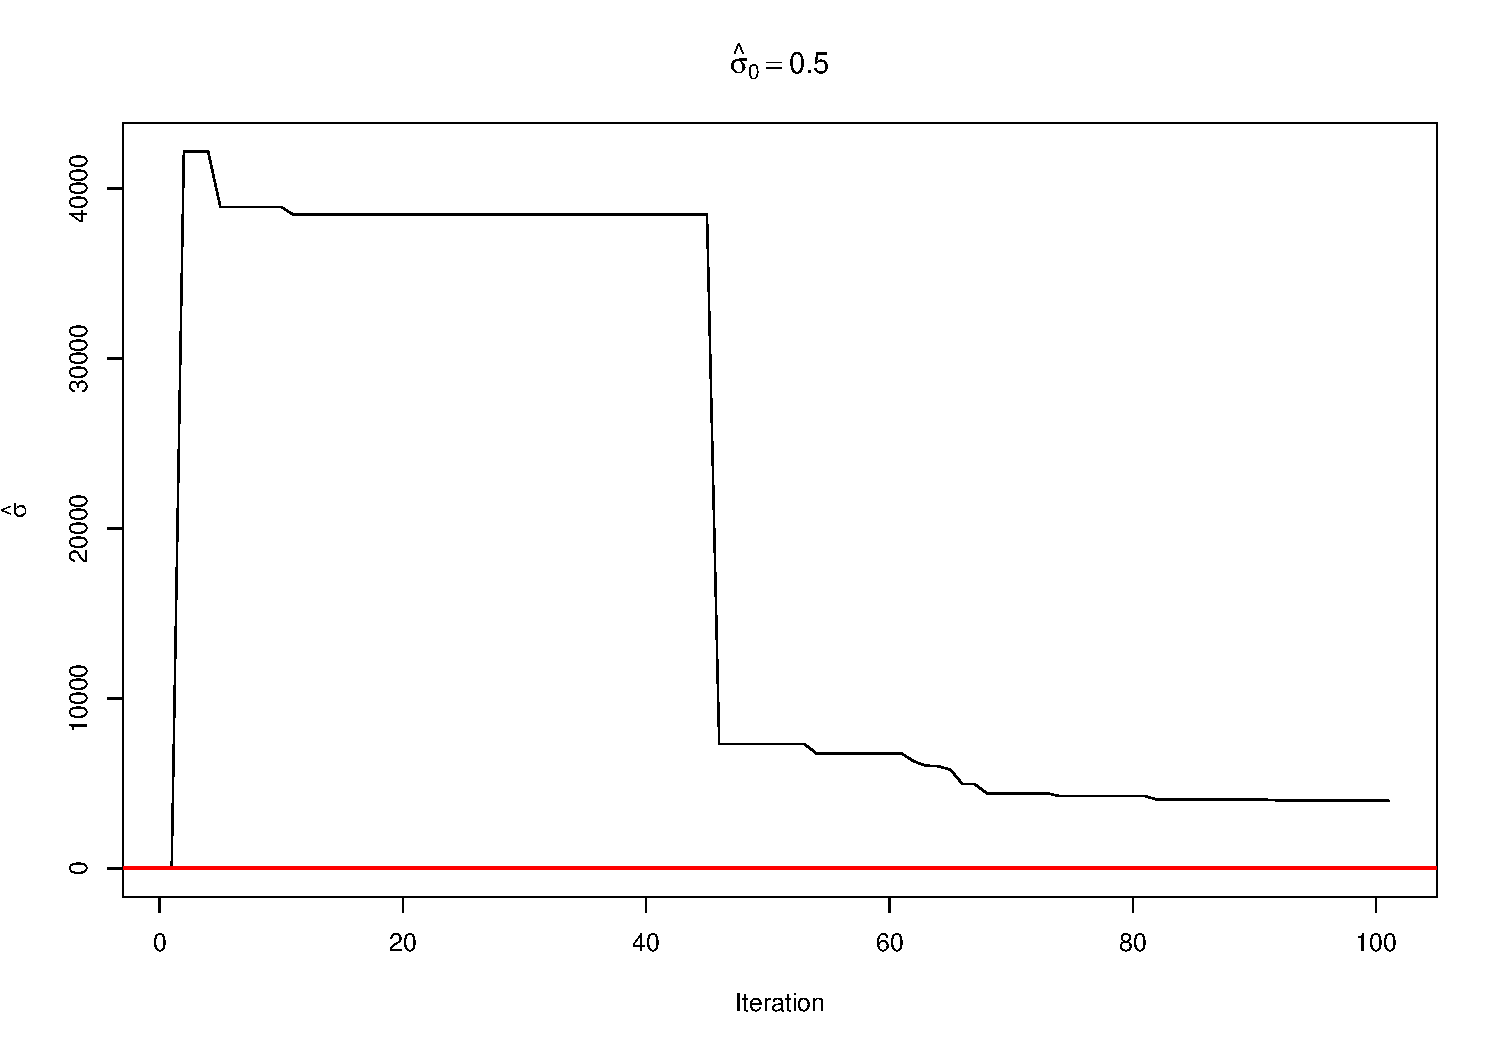
\includegraphics[height=0.9\textheight, width=0.9\textwidth, keepaspectratio]{Figures/ESS Traj - 0,5.pdf}
% \end{frame}

% \begin{frame}{Example: Mystery Target}
%     \centering
%     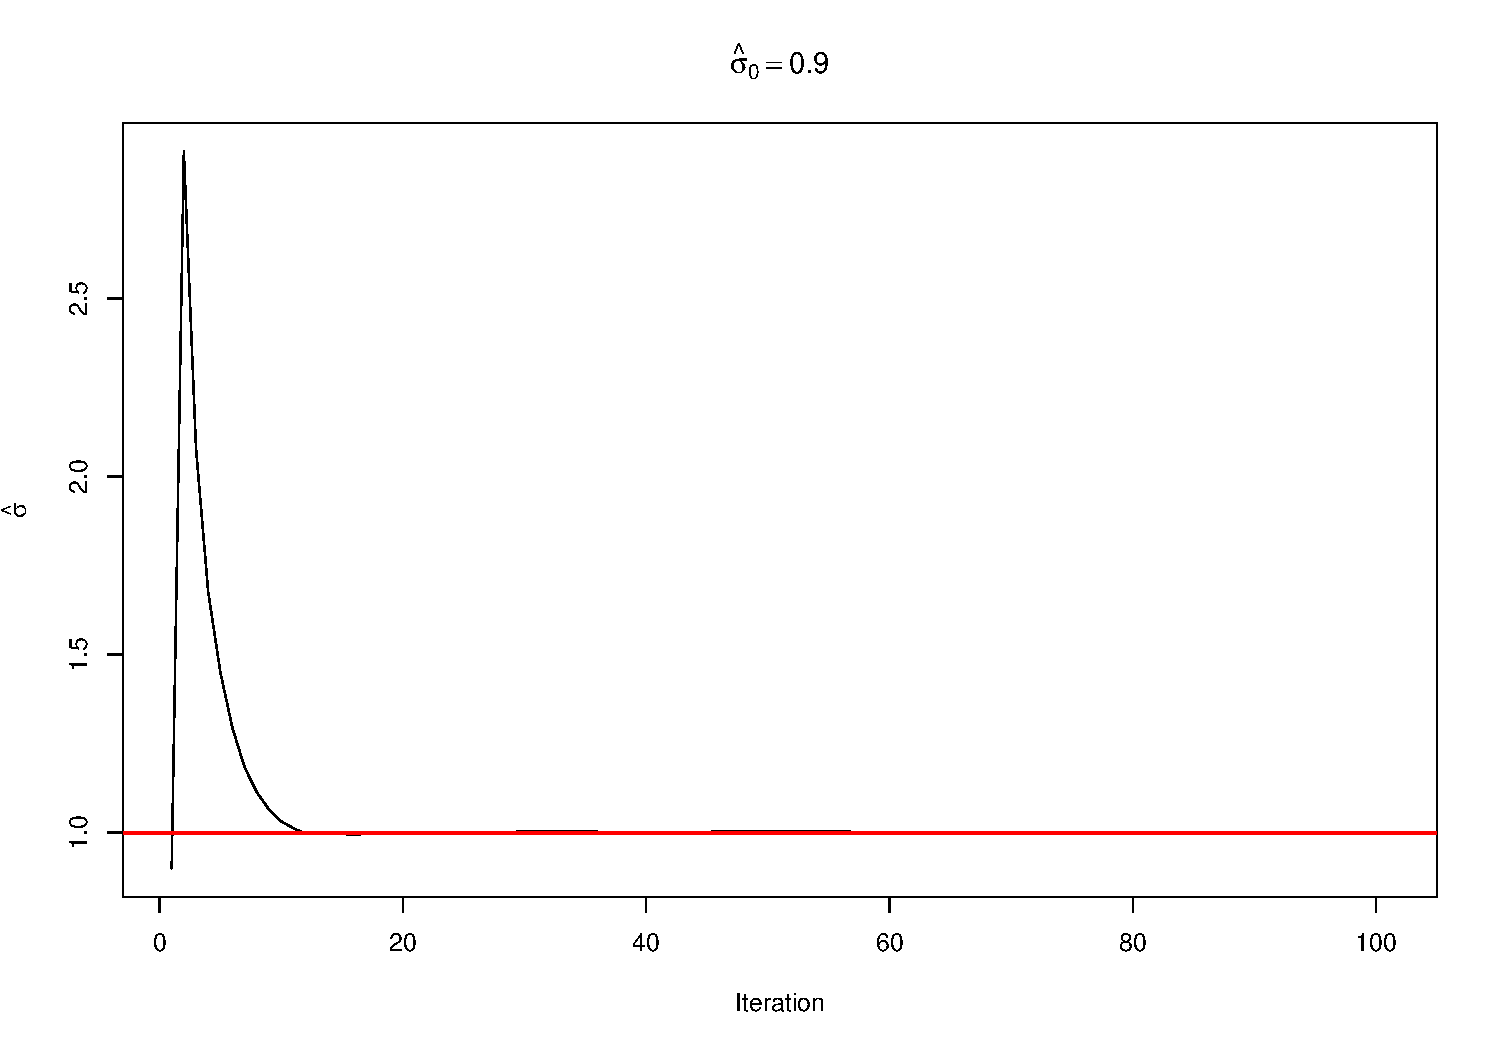
\includegraphics[height=0.9\textheight, width=0.9\textwidth, keepaspectratio]{Figures/ESS Traj - 0,9.pdf}
% \end{frame}

% \begin{frame}{Example: Mystery Target}
%     \centering
%     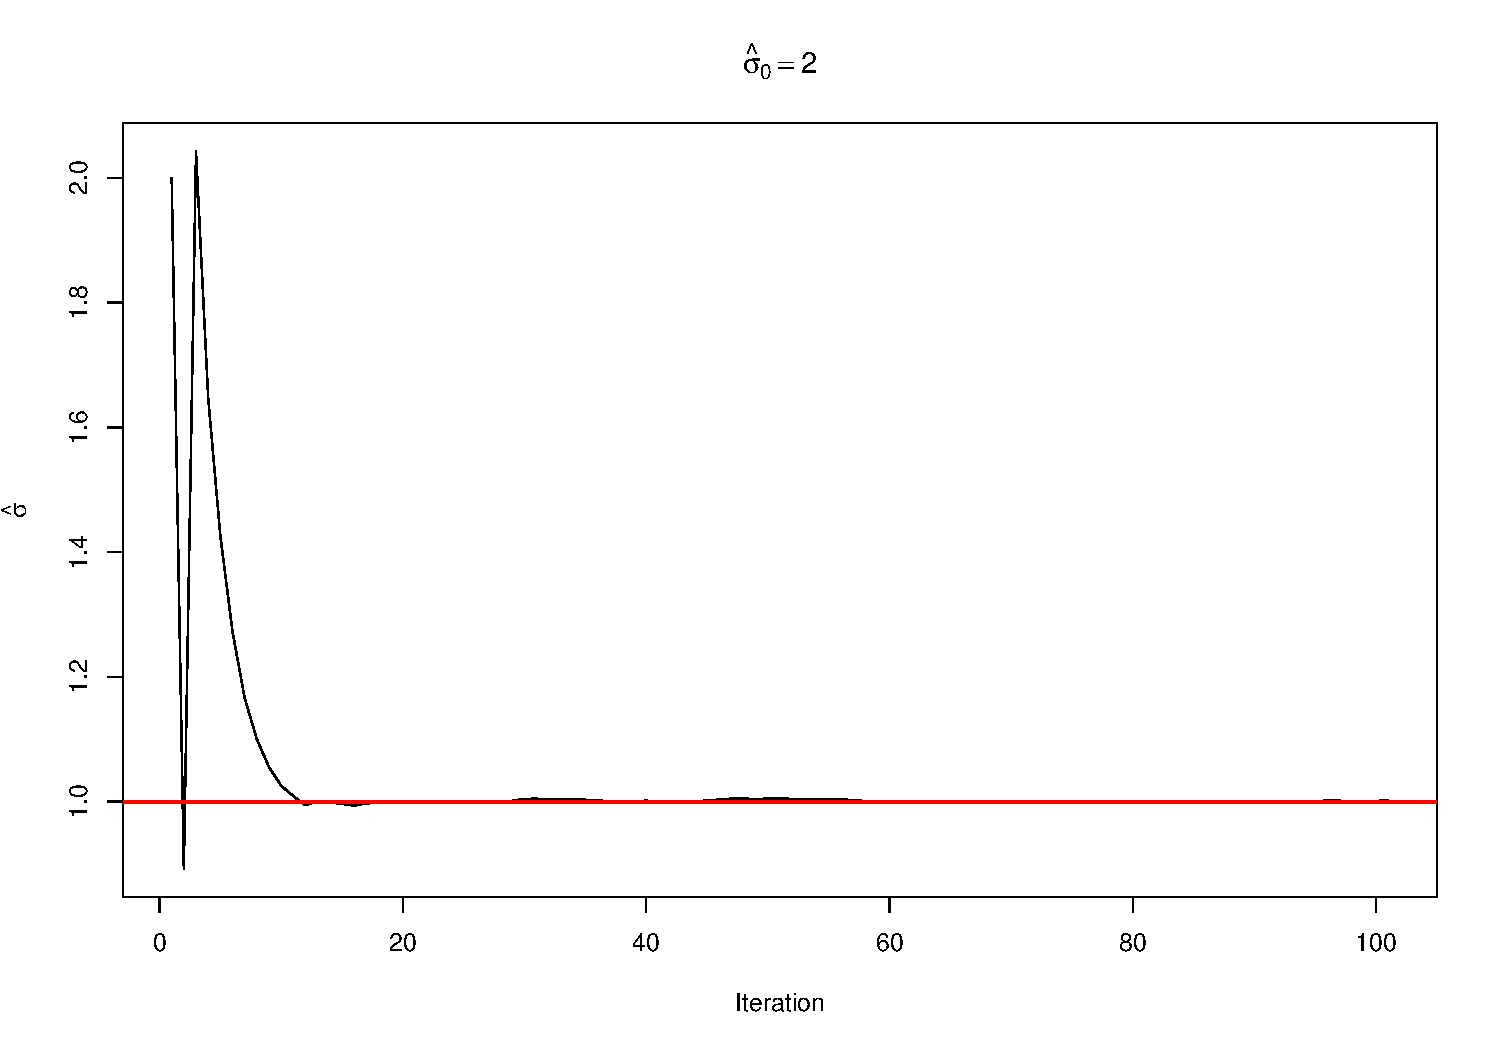
\includegraphics[height=0.9\textheight, width=0.9\textwidth, keepaspectratio]{Figures/ESS Traj - 2.pdf}
% \end{frame}

% \begin{frame}{Example: Mystery Target}
%     \centering
%     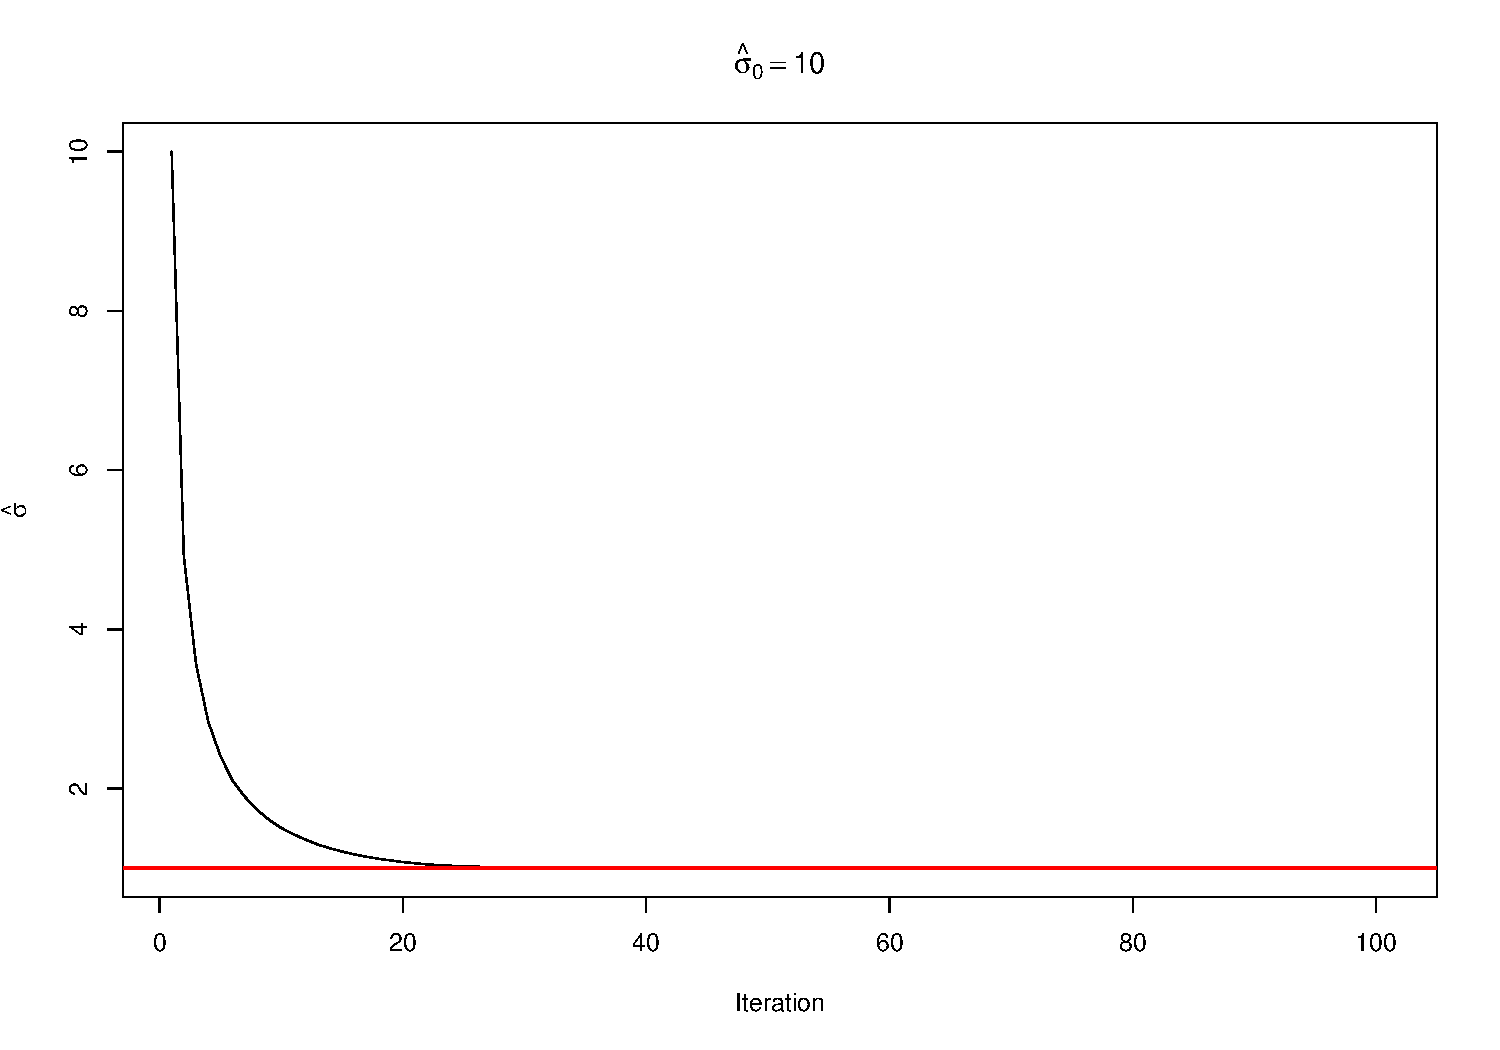
\includegraphics[height=0.9\textheight, width=0.9\textwidth, keepaspectratio]{Figures/ESS Traj - 10.pdf}
% \end{frame}


%! This resembles the previous slide
% \begin{frame}{Example: Mystery Target}
%     \centering
%     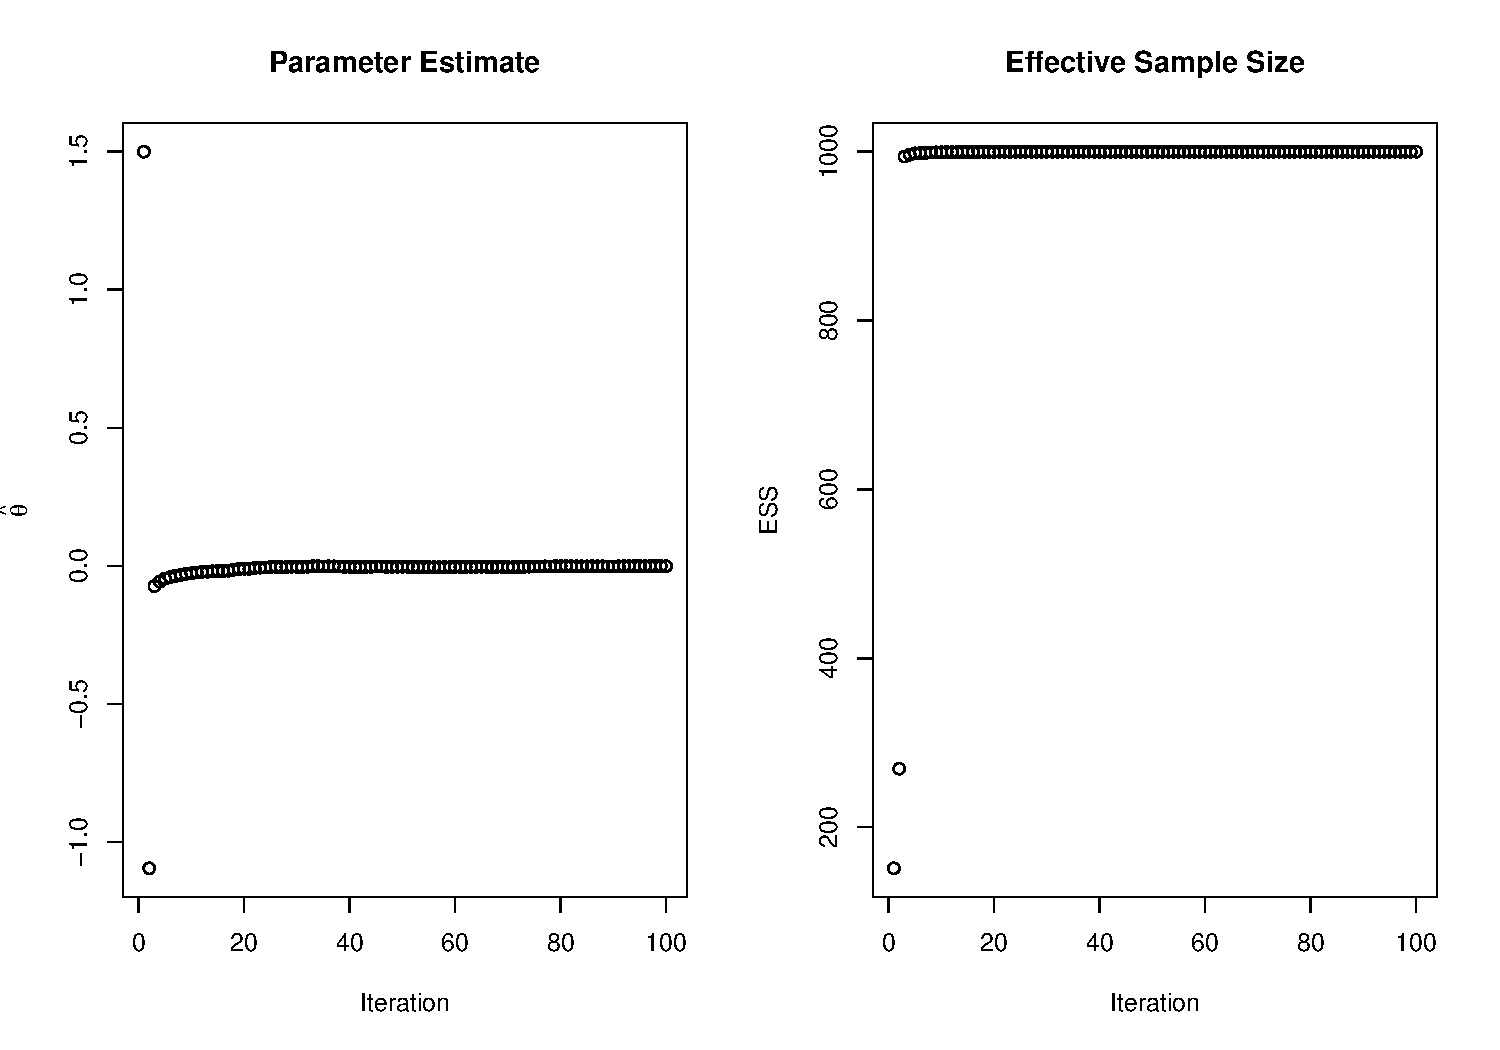
\includegraphics[height=0.7\textheight, width=0.9\textwidth, keepaspectratio]{Figures/ESS traj.pdf} \newline
%     \begin{outline}
%         $\hat{\theta}_\mathrm{end}^{(ESS)} \approx -8 \times 10^{-4}$ \hspace{1cm} $ESS_\mathrm{end} \approx 1000 - (7 \times 10^{-4})$
%     \end{outline}
% \end{frame}


\begin{frame}{Our Method}
    \begin{outline}
        \1 Recall: Be careful using IS means to diagnose IS \newline
        
        \1 \citeauthor{Veh22} give an alternative
            \2 Shape parameter of fitted tail distribution, $\hat{k}$
    \end{outline}
\end{frame}


%! Consider adding this back in. I haven't yet found a way to present the numerics that I feel confident about
% \begin{frame}{Our Method}
%     \begin{outline}
%         \1 Consider repeated sampling with $\sigma = 0.5$ (hard)
%         \1 For each sample, estimate $\rho$ and $k$ \newline

%         \1 Coefficient of Variation:
%             \2 $\hat{\rho}$: $5.06$
%             \2 $\hat{k}$: $0.22$
%     \end{outline}
    
% %     \centering
% %   \begin{tabular}{|c|c c|}
% %     \hline
% %     & $\hat{\rho}$ & $\hat{k}$ \\
% %     \hline
% %     Mean & 29.6 & 0.65 \\ 
% %     Standard Error & 15.0 & 0.01 \\ 
% %     Coefficient of Variation & {5.1} & {0.22}\\
% %     \hline
% %   \end{tabular}
% \end{frame}

% \begin{frame}{Our Method}
%     \centering
%   \begin{tabular}{|c|c c|}
%     \hline
%     & $\hat{\rho}$ & $\hat{k}$ \\
%     \hline
%     Mean & 29.6 & 0.65 \\ 
%     Standard Error & 15.0 & 0.01 \\ 
%     \textbf{Coefficient of Variation} & \textbf{5.1} & \textbf{0.22}\\
%     \hline
%   \end{tabular}
% \end{frame}

\begin{frame}{Our Method}
    \begin{outline}
        \1 Use diagnostic as objective function \newline

        \1 Apply stochastic approximation to minimize $\hat{k}$
            \2 More precisely, its population analog: $k(\theta)$ \newline

        \1 Use finite difference approximation to $\hat{k}'(\theta)$
            \2 This is subtle
    \end{outline}
\end{frame}

% \begin{frame}{Example: Mystery Target}
%     \centering
%     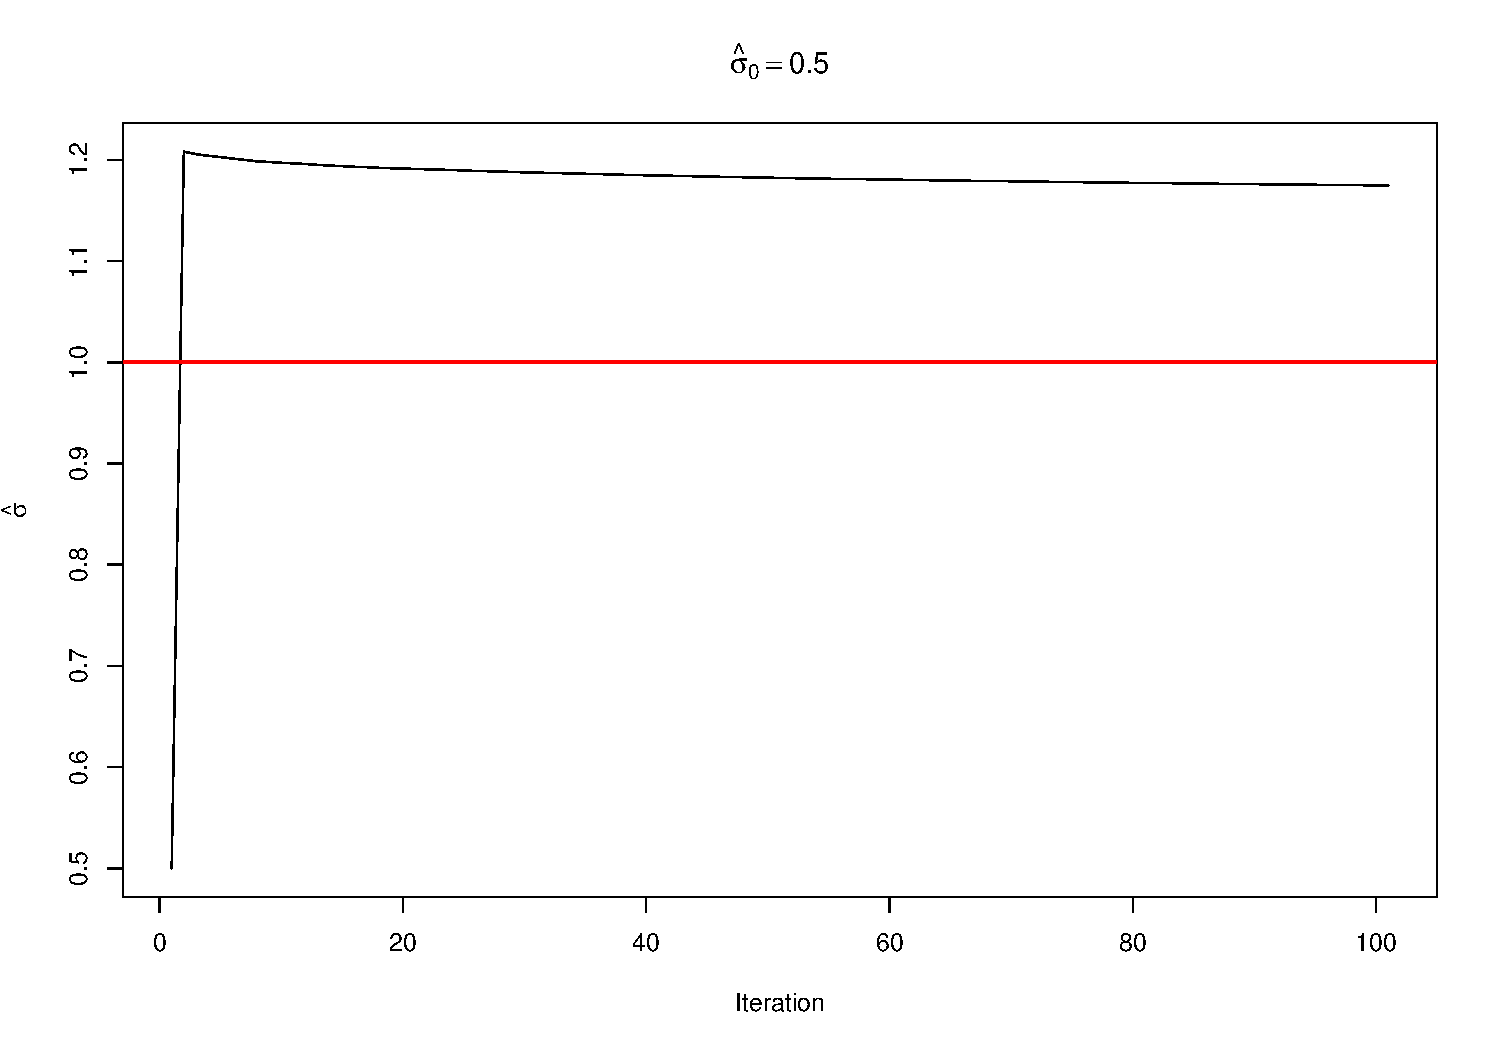
\includegraphics[height=0.9\textheight, width=0.9\textwidth, keepaspectratio]{Figures/k_hat Traj - 0,5.pdf}
% \end{frame}

% \begin{frame}{Example: Mystery Target}
%     \centering
%     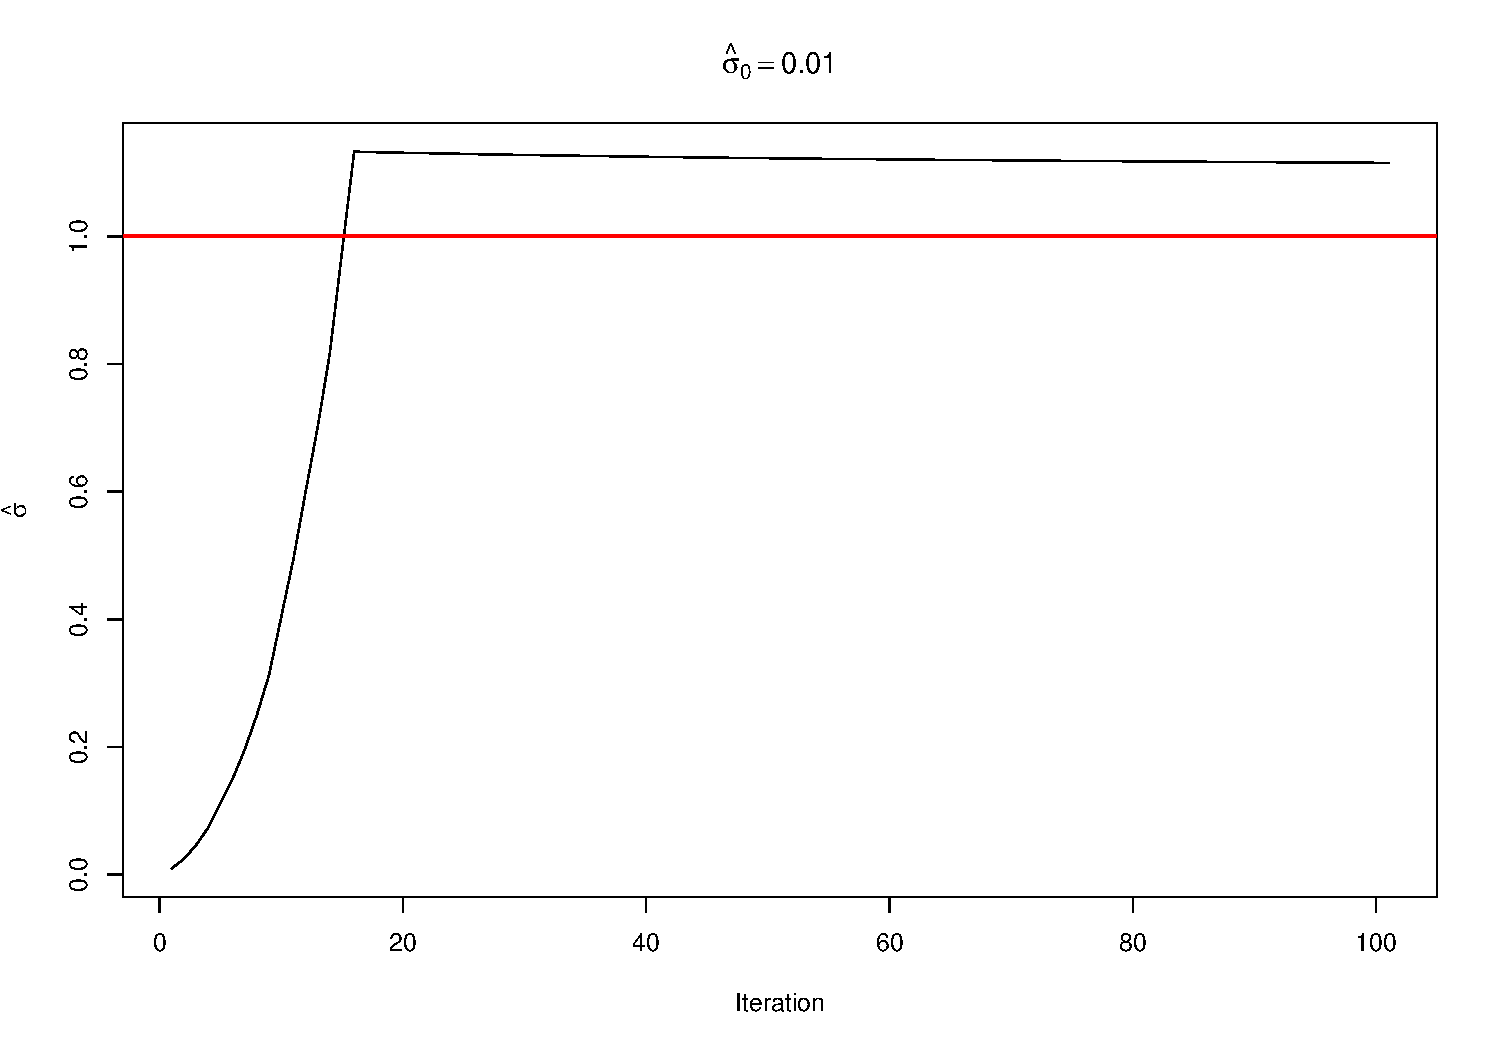
\includegraphics[height=0.9\textheight, width=0.9\textwidth, keepaspectratio]{Figures/k_hat Traj - 0,01.pdf}
% \end{frame}

% \begin{frame}{Example: Mystery Target}
%     \centering
%     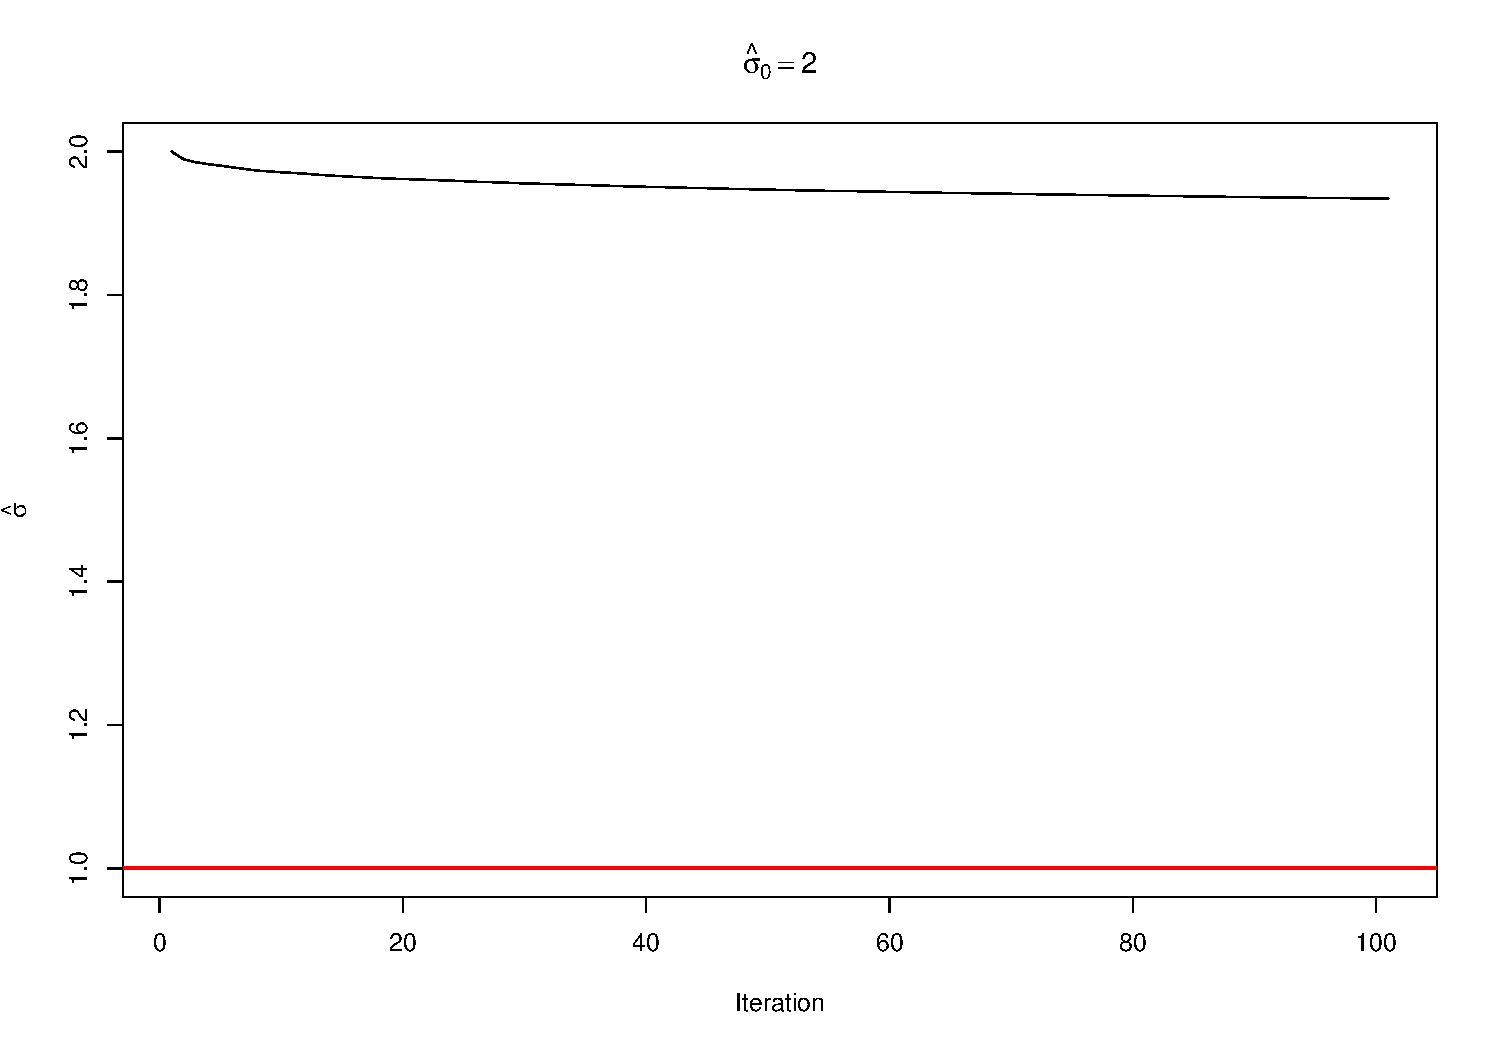
\includegraphics[height=0.9\textheight, width=0.9\textwidth, keepaspectratio]{Figures/k_hat Traj - 2.pdf}
% \end{frame}

\begin{frame}{Our Method - Future Directions}
    \begin{outline}
        \1 Refining the finite difference approximation
            \2 Generalize ESS version outside exponential families \newline

        \1 Analytical tail indices
        \1 Convergence theory for stochastic approximation \newline

        \1 Applications
            \2 Latent variable models (e.g. GLMMs)
            \2 Bayesian inference in high-dimensions
    \end{outline}
\end{frame}


\begin{frame}{Recap}
    \begin{outline}
        \1 Importance sampling and extensions
            \2 Truncation
            \2 Pareto Smoothing \newline
        
        \1 Diagnostics for importance sampling
            \2 Effective sample size
            \2 Pareto tail index \newline

        \1 Adaptive importance sampling
            \2 Stochastic approximation
    \end{outline}
\end{frame}



\end{comment}



%! Add Pictures?
\begin{frame}{Acknowledgements}
    \begin{outline}
        \1 Payman Nickchi (UBC)
        \1 Richard Lockhart (SFU)
    \end{outline}

\end{frame}



\begin{frame}
    \centering
    \Huge Thank You
\end{frame}

\begin{frame}{Some References}
    \bibliographystyle{apalike}
    \bibliography{Refs}
\end{frame}

\end{document}
